\setAuthor{Konstantis Dukatš}
\setRound{lõppvoor}
\setYear{2021}
\setNumber{G 9}
\setDifficulty{9}
\setTopic{TODO}

\prob{Vedelik peeglil}
Laua peal lebab veega täidetud sfääriline nõguspeegel, kusjuures vesi ulatub peegli servani (vt joonist). Peegli kohale kõrgusele $h=\SI{25.0}{cm}$ on kinnitatud valgusallikas nii, et selle kujutis kattub allikaga. Seejärel asendatakse vesi tundmatu vedelikuga, mille peale nihkub kujutis $l=\SI{5.0}{cm}$ võrra peegli poole. Leidke tundmatu vedeliku murdumisnäitaja. Eeldada, et peegli laius on palju väiksem kui $l$, $h$, s.t. võib kasutada väikeste nurkade lähendust $\sin \alpha \approx \tan \alpha \approx \alpha$, kus $\alpha$ on radiaanides. Vee murdumisnäitaja on $n_v=\num{1.33}$.
\begin{figure}[h]
  \centering
  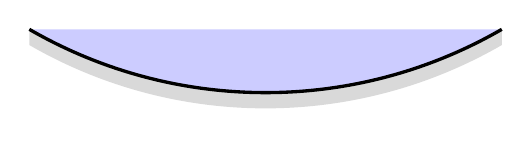
\begin{tikzpicture}
    \fill [fill opacity=0.2, fill=blue] (0,0) arc (240:300:6) -- (0,0) -- cycle;
    \fill [gray!30] (0,0) arc (240:300:6) -- ++(0,-0.2) arc (300:240:6) -- ++(0, 0.2) -- cycle;
    \draw [very thick] (0,0) arc (240:300:6);
  \end{tikzpicture}
\end{figure}
\vspace{-1.5em}


\hint

\solu
\emph{Lahendus 1.} Kui meil on vedelik kõvera peegli peal, käitub see vedelik nagu lääts, mille ühe poole kõverusraadius on sama peegli kõverusraadiusega ja teise poole kõverusraadius läheneb lõpmatusele. Kuna peegli laius on palju väikse kui $l,h$, siis on tegemist õhukese läätsega. Sellisel juhul läätse optiline tugevus
\[
  D_l=\frac{1}{f_l}=\frac{n-1}{R},
\]
kus $n$ on vedeliku murdumisnäitaja ja $R$ on peegli kõverusraadius\footnote{Tegu on läätsevalmistaja valemi erikujuga. Läätsevalmistaja valem annab üldjuhul sfääriliste pindadega läätse tugevuse:
  \[
    D=\frac{1}{f}=(n-1)\left[\frac{1}{R_1}-\frac{1}{R_2}+\frac{(n-1)d}{nR_1R_2}\right],
  \]
  kus $f$ on läätse fookuskaugus, $n$ on läätse materjali murdumisnäitaja õhu suhtes, $R_1$ on valgusallikale lähema pinna kõverusraadius (koos märgikonventsiooniga), $R_2$ on valgusallikale kaugema pinna kõverusraadius ja $d$ on läätse paksus.
}. Peegli optiline tugevus
\[
  D_p=\frac{1}{f_p}=\frac{2}{R},
\]
kus $f_p$ on peegli fookuskaugus. Kuna valguskiired läbivad läätse kaks korda (enne peegeldamist ja pärast), siis läätse tugevusega peab arvestama kaks korda. Konbineerides läätse ja peegli saame, et
\[
  \frac{1}{a}+\frac{1}{k}=2 D_l+D_p,
\]
kus $a$ on objekti kaugus läätsest ja peeglist ning $k$ on kujutise kaugus läätsest ja peeglist. Avaldades $D_l$ ja $D_p$ saame, et
\[
  \frac{1}{a}+\frac{1}{k}=\frac{2(n-1)}{R}+\frac{2}{R}=\frac{2n}{R}
\]
Vee korral
\[
  \frac{1}{h}+\frac{1}{h}=\frac{2 n_v }{R} \implies R=h n_v.
\]
Tundmatu vedeliku korral
\[
  \frac{1}{h}+\frac{1}{h-l}=\frac{2 n_x }{R}.
\]
Avaldades $n_x$ saame, et
\[
  n_x =\frac{(2h-l)}{2h(h-l)} R =\frac{(2h-l)}{2(h-l)} n_v \approx \num{1.50}.
\]

\emph{Lahendus 2.}
Vaatleme allikast tulevat kiirt, mis on vertikaali suhtes nurga $\alpha$ all. Järelikult siseneb kiir vedelikku kaugusel $a = \alpha h$ peegli sümmetriateljest. Snelli seaduse kohaselt on kiire nurk vertikaali suhtest peale vedelikku sisenemist $\frac{\alpha }{n}$. Olgu kiire nurk peale peegli vastu peegeldumist $\beta$. Väikeste nurkade lähenduses on peegli pinna normaal nurga $\frac{1}{2} (\frac{\alpha}{n} + \beta)$ all. Samas lõikub peegli pinna normaal sümmeetriateljega kaugusel $R$, kus $R$ on nõguspeegli kõverusraadius. Seega,
\[
  \frac{1}{2} \left(\frac{\alpha}{n} + \beta\right) = \frac{a}{R} = \frac{\alpha h}{R},
\]
järelikult
\[
  \beta = \frac{2\alpha h}{R} - \frac{\alpha}{n}.
\]
Edasi, pärast peegeldumist ning vedelikust järjekordset väljumist on kiire nurk vertikaali suhtes
\[
  \gamma = \beta n = \frac{2\alpha nh}{R} - \alpha.
\]
Seega saame, et kujutise kaugus peegli pinnast on
\[
  \frac{1}{d} = \frac{\gamma}{a} = \frac{\gamma}{\alpha h} = \frac{2n}{R}- \frac{1}{h}.
\]
Kasutades saadud seost esialgses olukorras näeme, et
\[
  \frac{1}{h} = \frac{2n_v}{R} - \frac{1}{h}.
\]
Teisisõnu, $R = n_v h$. Pärast tundmatu vedelikuga asendamist saame aga
\[
  \frac{1}{h - l} = \frac{2n}{R} - \frac{1}{h} = \frac{2n}{n_v h} - \frac{1}{h}.
\]
Järelikult
\[
  n = \frac{2h-l}{h - l}\cdot  \frac{n_v}{2} \approx \num{1.5}.
\]
\probend